\documentclass[11pt,a4paper]{article}
\usepackage[margin=0.85in,top=1in,bottom=1in]{geometry}
\usepackage{amsmath,amssymb,amsfonts}
\usepackage{graphicx}
\usepackage{float}
\usepackage{enumitem}
\usepackage{microtype}
\usepackage{caption}
\usepackage[hidelinks]{hyperref}
\usepackage[most,breakable]{tcolorbox}
\tcbuselibrary{breakable,skins}
\usepackage{fontspec}
\setmainfont{DejaVu Serif}
\setsansfont{DejaVu Sans}
\setmonofont{DejaVu Sans Mono}
\captionsetup{font=small,labelfont=bf,skip=4pt}
\setlist{leftmargin=1.5em,topsep=2pt}

%% Breakable problem card — prevents content cutoff across pages
\newtcolorbox{solcard}[3]{
  breakable, enhanced,
  colback=white, colframe=gray!50, arc=2pt,
  title={\textbf{#1}\hfill\textsf{\small #3\,pts}},
  fonttitle=\normalsize\sffamily\bfseries,
  before upper={\small\textit{#2}\par\smallskip\hrule height 0.4pt\smallskip},
  top=4pt, bottom=6pt, left=7pt, right=7pt,
  parbox=false,
}

\title{\textbf{Mixture viscosity measurement --- Solution}}
\author{\normalsize W26 (2026) — English translation}
\date{}
\begin{document}\maketitle\vspace{-0.5em}
\begin{solcard}{A1}{Express the mole fraction of water $n_w$ in solution in terms of the mass fraction of glycerol $w_g$, $\mu_w$ and $\mu_g$.}{0.20}

The amount of a substance in a mixture is defined as: \[\nu=\dfrac{m}{\mu},\] where $m$ is the mass of the substance, and $\mu$ is its molar mass. Let's write the formula for the molar concentration of water: \[n_w=1-n_g=1-\dfrac{\nu_g}{\nu_g+\nu_w},\] from here:


\[\nu=\dfrac{m}{\mu},\]


where $m$ is the mass of the substance, and $\mu$ is its molar mass.


Let's write the formula for the molar concentration of water:


\[n_w=1-n_g=1-\dfrac{\nu_g}{\nu_g+\nu_w},\]


from here:

\par\smallskip\noindent\textbf{Answer:} \textbackslash{}textbf{Answer:} \[n_w=1-\frac{w_g\mu_w}{\mu_g-w_g(\mu_g-\mu_w)}\]
\end{solcard}

\begin{solcard}{A2}{Using the equation $(1)$, convert the values ​​of $T_g$ to the values ​​of $w_g$.}{1.50}

Using the table method or the method of simple iterations with $a=0.9$, we get:

\par\smallskip\noindent\textbf{Answer:} \textbackslash{}textbf{Answer:} $T_g,~\mathrm{K}$ $w_g$ $\eta,~\mathrm{Pa}\cdotс$ 195.2 1.000 0.906 194.8 0.996 0.839 194.6 0.994 0.767 193.9 0.987 0.655 193.1 0.979 0.558 191.8 0.965 0.479 190.8 0.954 0.373 188.6 0.930 0.202 183.4 0.869 0.0674 173.0 0.728 0.0278 170.0 0.682 0.0134 154.6 0.384 0.0026 149.3 0.252 0.0017 143.8 0.100 0.0012 140.3 0 0.0009
\end{solcard}

\begin{solcard}{A3}{Propose a linearization that describes a system with a small mole fraction of water, which can be used to determine the parameters $\xi$ and $k$. Plot the linearized relationship. Determine the parameters $\xi$ and $k$ using the resulting graph.}{0.60}

Let's recalculate the points into the dependence $\operatorname{ln}\dfrac{\eta}{1~\mathrm{Pa}\cdot с}(n_w)$.


$T_g,~\mathrm{K}$ $w_g$ $\eta,~\mathrm{Pa}\cdotс$ $n_w$ $\operatorname{ln} \eta$ 195.2 1.000 0.906 0 -0.099 194.8 0.996 0.839 0.020 -0.176 194.6 0.994 0.767 0.030 -0.265 193.9 0.987 0.655 0.063 -0.423 193.1 0.979 0.558 0.099 -0.583 191.8 0.965 0.479 0.156 -0.736 190.8 0.954 0.373 0.198 -0.986 188.6 0.930 0.202 0.278 -1.600 183.4 0.869 0.0674 173.0 0.728 0.0278 170.0 0.682 0.0134 154.6 0.384 0.0026 149.3 0.252 0.0017 143.8 0.100 0.0012 140.3 0 0.0009


Let's plot the resulting dependence in the range $n_w \in [0, 0.2]$.


$\operatorname{ln}\dfrac{\eta}{1~\mathrm{Pa}\cdot с}(n_w)$


Approximating the dependence of the straight line, we obtain: \[k=4.31,\] \[\operatorname{ln}\dfrac{\xi}{1~\mathrm{Pa}\cdot с}=-0.12,\]from which it follows:

\par\smallskip\noindent\textbf{Answer:} \textbackslash{}textbf{Answer:} \[k=4.31\]\[\xi=0.887~\mathrm{Pa}\cdot с\]
\begin{figure}[H]
  \centering
  
\includegraphics[width=0.72\textwidth]{PE+_S_EN_assets/fig1.jpg}
\end{figure}
\end{solcard}

\begin{solcard}{A4}{Knowing the parameters $\xi$ and $k$, propose a linearization that allows you to determine the values ​​of the parameters $a$ and $b$. Plot the linearized relationship. Using the straight section, determine $a$ and $b$.}{0.50}

Let's continue recalculating points:


$T_g,~\mathrm{K}$ $w_g$ $\eta,~\mathrm{Pa}\cdotс$ $n_w$ $\operatorname{ln}|\dfrac{\xi \operatorname{exp}(-kn_w)}{\eta}-1|$ 195.2 1.000 0.906 0 -3.92 194.8 0.996 0.839 0.020 -3.54 194.6 0.994 0.767 0.030 -4.12 193.9 0.987 0.655 0.063 -3.44 193.1 0.979 0.558 0.099 -3.28 191.8 0.965 0.479 0.156 -2.91 190.8 0.954 0.373 0.198 -4.35 188.6 0.930 0.202 0.278 -1.12 183.4 0.869 0.0674 0.435 0.02 173.0 0.728 0.0278 0.656 -0.12 170.0 0.682 0.0134 0.704 0.78 154.6 0.384 0.0026 0.891 1.85 149.3 0.252 0.0017 0.938 2.10 143.8 0.100 0.0012 0.979 2.29 140.3 0 0.0009 1 2.50


Let's plot the resulting points on the graph:


$\operatorname{ln}|\dfrac{\xi \operatorname{exp}(-kn_w)}{\eta}-1|(n_w)$


In the range $n_w \in [0, 0.2]$, the expression under the logarithm has a different sign and is near zero, so the function in this region behaves non-monotonic. To draw a straight line, we take into account only points in the range $n_w \in [0.7, 1].$


$\operatorname{ln}|\dfrac{\xi \operatorname{exp}(-kn_w)}{\eta}-1|(n_w)$ in the range $n_w \in [0.7, 1]$ (not required from participants)


For $n_w>0.2$, $\dfrac{\xi \operatorname{exp}(-kn_w)}{\eta}>1$ holds, so $a>0$. Having drawn the approximating straight line, we find: \[b=5.66,\]\[\operatorname {ln} a=-3.21,\]from here:

\par\smallskip\noindent\textbf{Answer:} \textbackslash{}textbf{Answer:} \[a=0.040\]\[b=5.66\]
\begin{figure}[H]
  \centering
  
\includegraphics[width=0.72\textwidth]{PE+_S_EN_assets/fig2.jpg}
\end{figure}
\begin{figure}[H]
  \centering
  
\includegraphics[width=0.72\textwidth]{PE+_S_EN_assets/fig3.jpg}
\end{figure}
\end{solcard}

\begin{solcard}{A5}{Draw a graph of the theoretical and experimental dependence $\eta(n_w)$ on one piece of graph paper. Indicate the range of applicability of the resulting equation.}{0.70}

Let's calculate the values ​​of the theoretical dependence $\eta(n_w)$:


$T_g,~\mathrm{K}$ $w_g$ $\eta,~\mathrm{Pa}\cdotс$ $n_w$ $\operatorname{ln} \eta$ $\operatorname{ln}|\dfrac{\xi \operatorname{exp}(-kn_w)}{\eta}-1|$ $\eta_{теор},~\mathrm{Pa}\cdotс$ 195.2 1.000 0.906 0 -0.099 -3.92 0.853 194.8 0.996 0.839 0.020 -0.176 -3.54 0.779 194.6 0.994 0.767 0.030 -0.265 -4.12 0.744 193.9 0.987 0.655 0.063 -0.423 -3.44 0.640 193.1 0.979 0.558 0.099 -0.583 -3.28 0.541 191.8 0.965 0.479 0.156 -0.736 -2.91 0.413 190.8 0.954 0.373 0.198 -0.986 -4.35 0.337 188.6 0.930 0.202 0.278 -1.600 -1.12 0.224 183.4 0.869 0.0674 0.435 0.02 0.0926 173.0 0.728 0.0278 0.656 -0.12 0.0199 170.0 0.682 0.0134 0.704 0.78 0.0135 154.6 0.384 0.0026 0.891 1.85 0.0026 149.3 0.252 0.0017 0.938 2.10 0.0017 143.8 0.100 0.0012 0.979 2.29 0.0012 140.3 0 0.0009 1 2.50 0.0010


Let's build a graph of the obtained dependencies:


$\eta(n_w)$


Having drawn smoothing curves, we conclude:

\par\smallskip\noindent\textbf{Answer:} \textbackslash{}textbf{Answer:} The equation is applicable over the entire range ($n_w \in [0, 1]$).
\begin{figure}[H]
  \centering
  
\includegraphics[width=0.72\textwidth]{PE+_S_EN_assets/fig4.jpg}
\end{figure}
\end{solcard}

\begin{solcard}{B1}{Using the equation $(2)$, determine the glass transition temperature of the solution.}{0.40}

Let's express $w_g$: \[w_g=\dfrac{m_g}{m_g+m_w}=\dfrac{\rho_gc_g}{(\rho_g-\rho_w)c_g+\rho_w},\] then:

\par\smallskip\noindent\textbf{Answer:} \textbackslash{}textbf{Answer:} $T_g=(140.3+35.272\dfrac{\rho_gc_g}{(\rho_g-\rho_w)c_g+\rho_w}-3.879(\dfrac{\rho_gc_g}{(\rho_g-\rho_w)c_g+\rho_w})^2+23.467(\dfrac{\rho_gc_g}{(\rho_g-\rho_w)c_g+\rho_w})^3)K\approx 162.8~K$
\end{solcard}

\begin{solcard}{B2}{Propose a linearization to determine the values ​​of the parameters $D$ and $T_0$. By plotting a linearized relationship or using the least squares method (OLS), determine the parameter values.}{1.50}

The dependence $\dfrac{1}{\operatorname {ln}\dfrac{\eta}{\eta_0}}(T)$ is linear with slope $k=\dfrac{1}{DT_0}$ and intercept term $b=-\dfrac{1}{D}$. Let’s recalculate the point using this formula and plot the linearized dependence:


$T,~^\circ C$ $\eta,~\mathrm{Pa}\cdotс$ $T,~\mathrm{K}$ $\dfrac{1}{\operatorname{ln}\dfrac{\eta}{\eta_0}}$ 1 0.0201 274 0.1149 4 0.0173 277 0.1169 11 0.0128 284 0.1212 15 0.0104 288 0.1243 35 0.0046 308 0.1383 44 0.0034 317 0.1443 50 0.0031 323 0.1463 56 0.0026 329 0.1501 60 0.0022 333 0.1540 67 0.0020 340 0.1563 71 0.0017 344 0.1604 76 0.00145 349 0.1646 85 0.0013 358 0.1676 90 0.0011 363 0.1724 96 0.0010 369 0.1753 100 0.0009 373 0.1786


$\dfrac{1}{\operatorname{ln}\dfrac{\eta}{\eta_0}}(T)$


Having determined the parameters of the approximating straight line, we obtain a system of equations: \[\begin{cases}-\dfrac{1}{D}=-0.059\\ \dfrac{1}{DT_0}=6.38\cdot 10^{-4} К^{-1},\end{cases}\] which follows:

\par\smallskip\noindent\textbf{Answer:} \textbackslash{}textbf{Answer:} \[T_0=92.5~\mathrm{K}\]\[D=16.9\]
\begin{figure}[H]
  \centering
  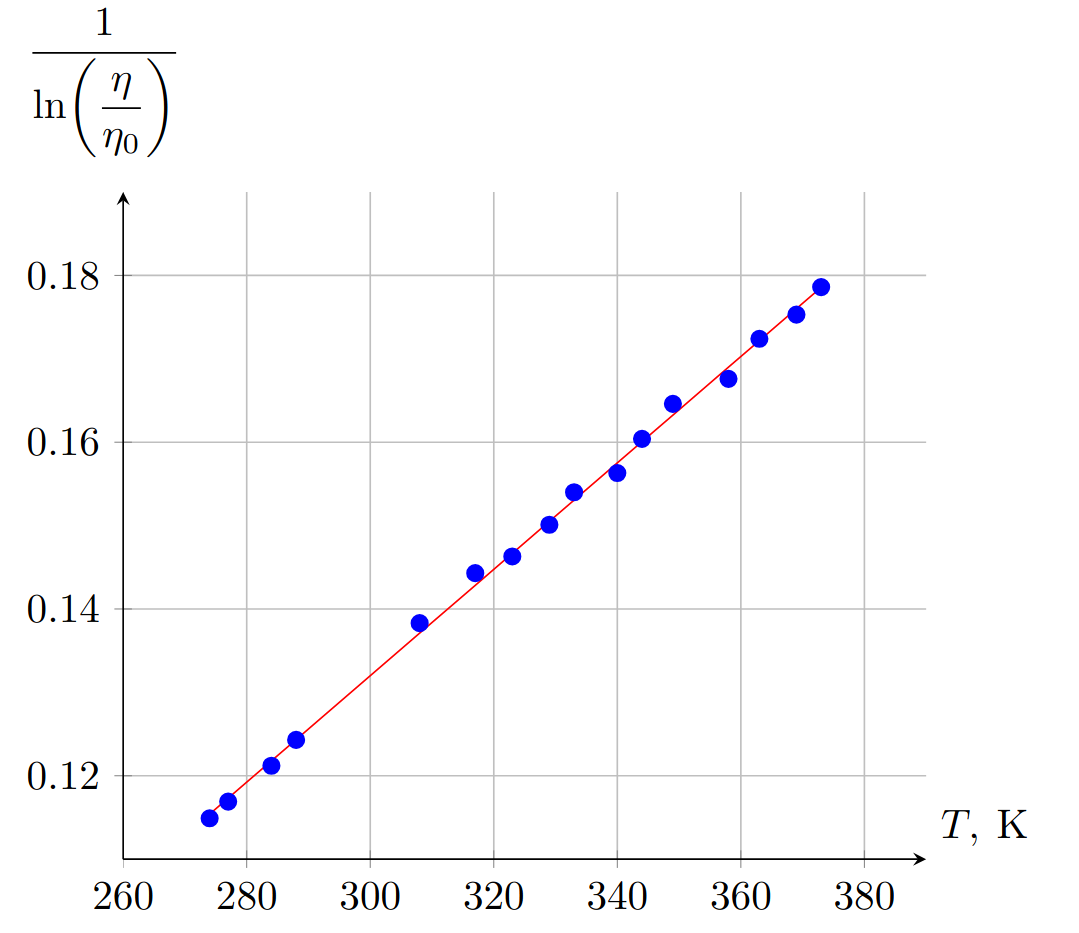
\includegraphics[width=0.72\textwidth]{PE+_S_EN_assets/fig5.jpg}
\end{figure}
\end{solcard}

\begin{solcard}{C1}{Determine the viscosity of the mixture $\eta_n$ at the volume fraction of glycerol $c_g=0.5$ and temperature $T=25~^\circ \mathrm C$ using the dependence on the mole fraction of water.}{0.30}

The equation obtained for $\eta_n(n_w)$ is applicable over the entire range. Therefore, it is enough to convert $c_g$ into $n_w$: \[n_w=1-\frac{w_g\mu_w}{\mu_g-w_g(\mu_g-\mu_w)}=1-\frac{\dfrac{\rho_gc_g}{(\rho_g-\rho_w)c_g+\rho_w}\mu_w}{\mu_g-\dfrac{\rho_gc_g}{(\rho_g-\rho_w)c_g+\rho_w}(\mu_g-\mu_w)}\approx 0.80\] and substitute it into the resulting equation. Thus we get:

\par\smallskip\noindent\textbf{Answer:} \textbackslash{}textbf{Answer:} $\eta_n=6.0~\mathrm{m}Па\cdot с$
\end{solcard}

\begin{solcard}{C2}{Determine the viscosity of the mixture $\eta_t$ under the same conditions using the temperature dependence.}{0.30}

Similar to the previous point, we substitute the value $T=25^\circ~C=298~\mathrm{K}$ into the equation obtained in part B, which follows:

\par\smallskip\noindent\textbf{Answer:} \textbackslash{}textbf{Answer:} $\eta_t=6.8~\mathrm{m}Па\cdot с$
\end{solcard}

\begin{solcard}{C3}{Compare your results. If there are discrepancies, explain the reason for them.}{0.20}
\par\smallskip\noindent\textbf{Answer:} \textbackslash{}textbf{Answer:} Considering that the measurement range is large, the results can be considered coincident. The slight difference is most likely due to inaccurate temperature measurements, since the dependence of viscosity on temperature is very strong.
\end{solcard}

\begin{solcard}{D1}{Restore the missing values ​​$v_2$ in the table. Use the linearized dependence graph $v_2(\eta)$ for this. Use the empty table columns on the answer sheet to convert the required values.}{2.00}

In the case of a hydrophilic capillary, the dependence of the volumetric flow rate of liquid on viscosity is represented by the equation: \[Q=\pi r^2 v=\dfrac{\pi r^4 \Delta P}{8\eta L}=\dfrac{\pi r^4 \rho g}{8\eta }\], which implies the relation: \[v=k\dfrac{\rho}{\eta},\] where $k$ is a constant value. The density of the mixture can be calculated as: \[\rho=\rho_g c_g+\rho_w c_w=\rho_w+(\rho_g-\rho_w)c_g\] Using the expression: \[n_w=1-\frac{\dfrac{\rho_gc_g}{(\rho_g-\rho_w)c_g+\rho_w}\mu_w}{\mu_g-\dfrac{\rho_gc_g}{(\rho_g-\rho_w)c_g+\rho_w}(\mu_g-\mu_w)},\] we express $c_g$: \[n_w(\mu_g\rho_w(1-c_g)+\rho_g c_g\mu_w)=\mu_g\rho_w(1-c_g)\] \[c_g=\dfrac{\mu_g\rho_w(1-n_w)}{\rho_g\mu_w+\rho_w\mu_g(1-n_w)}\] Then the expression for the density of the mixture becomes: \[\rho=\rho_w+(\rho_g-\rho_w)\dfrac{\mu_g\rho_w(1-n_w)}{\rho_g\mu_w+\rho_w\mu_g(1-n_w)}\] Using the results of part A, we numerically determine the values of $n_w$ at $\eta<\xi$, then calculate the values of the densities of mixtures, then for each value velocity in the hydrophilic channel, we calculate the value of quantity $\dfrac{\rho}{\eta}$ and plot graph $v\left(\dfrac{\rho}{\eta}\right)$:


$\eta,~\mathrm{m}Па\cdotс$ $v_1,~\mathrm{\mu{}m}/с$ $v_2,~\mathrm{mm}/с$ $n_w$ $\rho, ~\dfrac{kg}{м^3}$ $\rho/\eta, ~\dfrac{\mathrm{s}}{м^2}\cdot 10^3$ 0.95 4.25 649 1.000 1000 1050 1.18 4.86 602 0.978 1021 865 1.32 5.03 545 0.966 1032 782 1.92 8.03 408 0.926 1060 552 2.41 9.80 310 0.905 1072 445 3.95 15.2 285 0.847 1100 278 5.81 18.2 253 0.804 1115 192 13.2 24.3 185 0.707 1141 86.4 18.4 25.5 0.666 1150 62.5 24.8 29.3 0.627 1157 46.7 72.3 38.8 0.475 1177 16.3 78.0 40.3 0.463 1178 15.1 224 51.0 0.278 1194 5.33 515 55.3 0.110 1204 2.34 989 59.4 1260 1.27 1400 65.2 1260 0.900


$v\left(\dfrac{\rho}{\eta}\right)$


The straight line must pass through $(0, 0)$, therefore, drawing it along 4 points, we find $k$: \[k=0.674\cdot 10^{-6}~\dfrac{м^3}{с^2}\]Now knowing $k$, we can restore the dependence $v_2(\eta)$:


$\eta,~\mathrm{m}Па\cdotс$ $v_1,~\mathrm{\mu{}m}/с$ $v_2,~\mathrm{mm}/с$ $n_w$ $\rho, ~\dfrac{kg}{м^3}$ $\rho/\eta, ~\dfrac{\mathrm{s}}{м^2}\cdot 10^3$ 0.95 42.5 649 1.000 1000 1050 1.18 48.6 602 0.978 1021 865 1.32 50.3 545 0.966 1032 782 1.92 80.3 408 0.926 1060 552 2.41 98.0 310 0.905 1072 445 3.95 152 285 0.847 1100 278 5.81 182 253 0.804 1115 192 13.2 243 185 0.707 1141 86.4 18.4 255 42.2 0.666 1150 62.5 24.8 293 31.5 0.627 1157 46.7 72.3 388 11.0 0.475 1177 16.3 78.0 403 10.2 0.463 1178 15.1 224 510 3.59 0.278 1194 5.33 515 553 1.58 0.110 1204 2.34 989 594 0.856 1260 1.27 1400 652 0.607 1260 0.900

\begin{figure}[H]
  \centering
  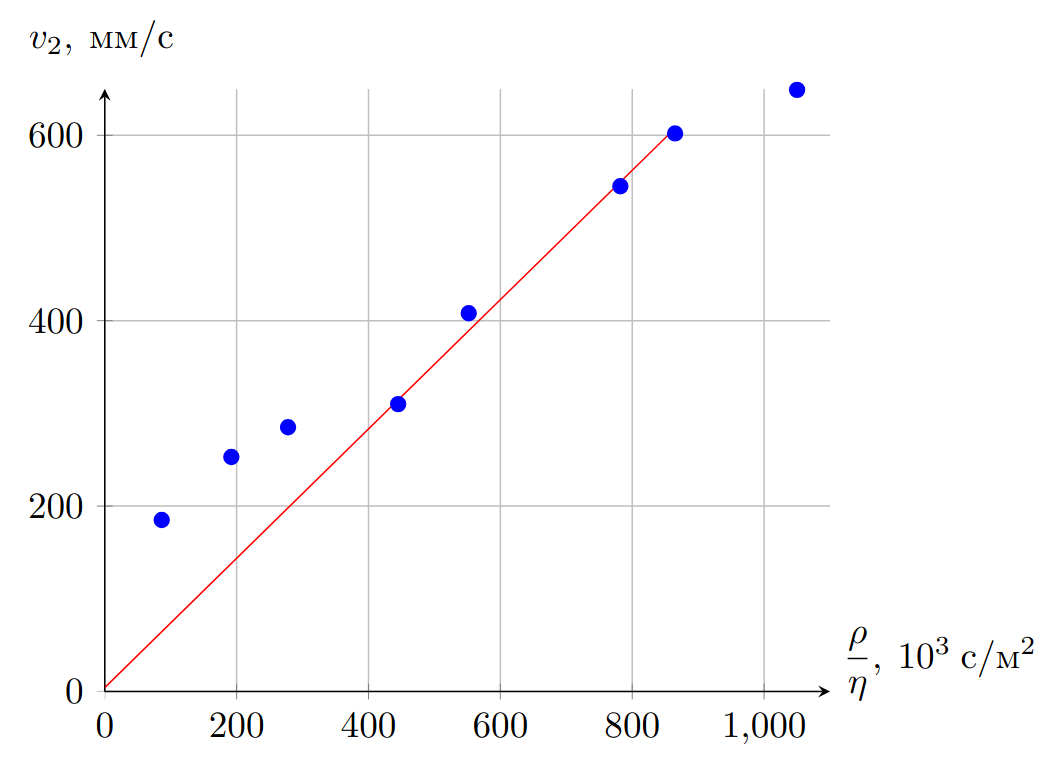
\includegraphics[width=0.72\textwidth]{PE+_S_EN_assets/fig6.jpg}
\end{figure}
\end{solcard}

\begin{solcard}{D2}{Construct a graph of $v_1(\eta)$ in the range from $\eta_1=10^{-3}~\mathrm{Pa}\cdot с$ to $\eta_2=10^{3}~\mathrm{Pa}\cdot с$ in the coordinates that are most convenient for graphical analysis. All points plotted on the graph must be tabulated on the answer sheet.}{1.50}

At high viscosities, the velocities in hydrophobic and hydrophilic capillaries are equal, at $\eta=1.400~\mathrm{Pa}\cdot с$ $v_1>v_2$, therefore we further assume that $v_1=v_2$ at $\eta>\eta_{max}=1.400~\mathrm{Pa}\cdot с$. Let's enter the points into the table and construct a graph in logarithmic coordinates, since the values ​​of the quantities under study vary by several orders of magnitude.


$\eta,~\mathrm{m}Па\cdotс$ $v_1,~\mathrm{\mu{}m}/с$ $v_2,~\mathrm{mm}/с$ $n_w$ $\rho, ~\dfrac{kg}{м^3}$ $\rho/\eta, ~\dfrac{\mathrm{s}}{м^2}\cdot 10^3$ $\operatorname{ln}\dfrac{v}{1~\mathrm{mm}/с}$ $\operatorname{ln}\dfrac{\eta}{1~\mathrm{Pa}\cdot с}$ 0.95 42.5 649 1.000 1000 1050 3.75 -6.96 1.18 48.6 602 0.978 1021 865 3.88 -6.74 1.32 50.3 545 0.966 1032 782 3.92 -6.63 1.92 80.3 408 0.926 1060 552 4.39 -6.26 2.41 98.0 310 0.905 1072 445 4.58 -6.03 3.95 152 285 0.847 1100 278 5.02 -5.53 5.81 182 253 0.804 1115 192 5.20 -5.15 13.2 243 185 0.707 1141 86.4 5.49 -4.33 18.4 255 42.2 0.666 1150 62.5 5.54 -4.00 24.8 293 31.5 0.627 1157 46.7 5.68 -3.70 72.3 388 11.0 0.475 1177 16.3 5.96 -2.63 78.0 403 10.2 0.463 1178 15.1 6.00 -2.55 224 510 3.59 0.278 1194 5.33 6.23 -1.50 515 553 1.58 0.110 1204 2.34 6.32 -0.66 989 594 0.856 1260 1.27 6.39 -0.01 1400 652 0.607 1260 0.900 6.48 0.34 $\eta,~\mathrm{Pa}\cdotс$ $v_1,~\mathrm{\mu{}m}/с$ $v_2,~\mathrm{mm}/с$ $n_w$ $\rho, ~\dfrac{kg}{м^3}$ $\rho/\eta, ~\dfrac{\mathrm{s}}{м^2}$ $\operatorname{ln}\dfrac{v_1}{1~\mathrm{\mu{}m}/с}$ $\operatorname{ln}\dfrac{\eta}{1~\mathrm{Pa}\cdot с}$ 2.5 340 1260 504 5.83 0.92 5.0 170 1260 252 5.14 1.61 10.0 84.9 1260 126 4.44 2.30 25.0 34.0 1260 50.4 3.53 3.22 50.0 17.0 1260 25.2 2.83 3.92 100 8.49 1260 12.6 2.14 4.61 200 4.25 1260 6.30 1.45 5.30 500 1.70 1260 2.52 0.53 6.21 1000 0.85 1260 1.26 -0.16 6.91


Let's plot the obtained points on the graph:


$\operatorname{ln}\dfrac{v_1}{1~\mathrm{\mu{}m}/с}\left(\operatorname{ln}\dfrac{\eta}{1~\mathrm{Pa}\cdot с}\right)$

\begin{figure}[H]
  \centering
  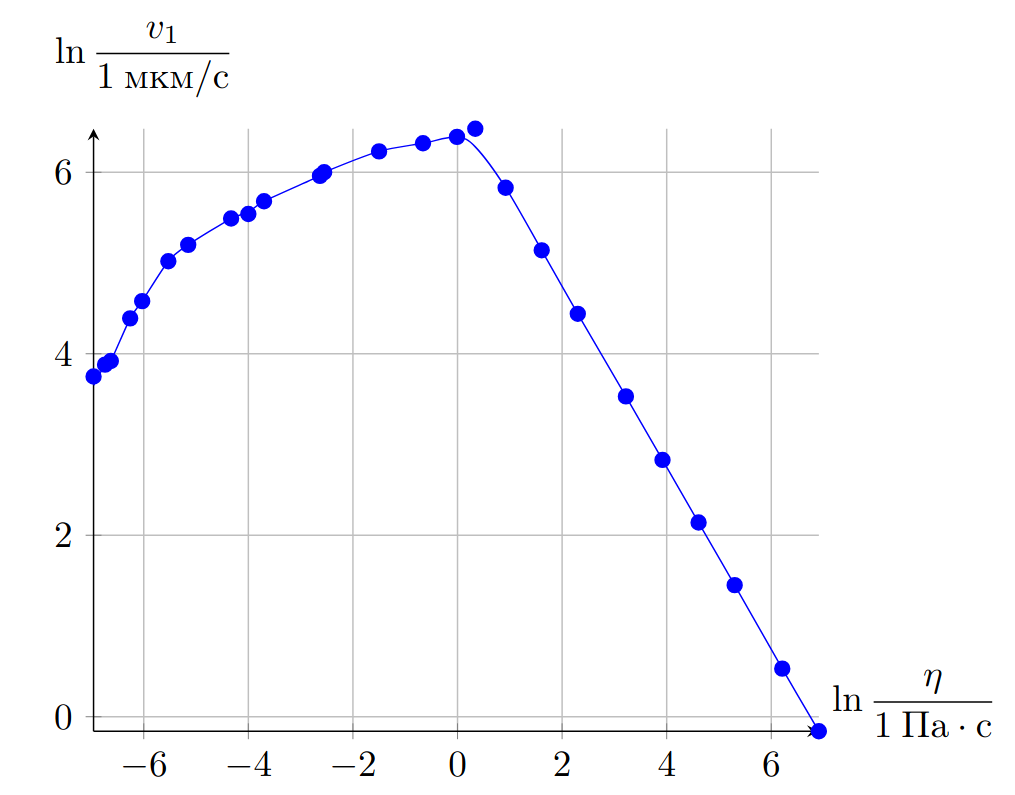
\includegraphics[width=0.72\textwidth]{PE+_S_EN_assets/fig7.jpg}
\end{figure}
\end{solcard}

\begin{solcard}{D3}{Determine the value of the mixture viscosity $\eta_{max}$ such that the value $v_2(\eta_{max})$ is maximum.}{0.30}
\par\smallskip\noindent\textbf{Answer:} \textbackslash{}textbf{Answer:} \[\eta_{max}=1.400~\mathrm{Pa}\cdot с\]
\end{solcard}

\end{document}